%%%%%%%%%%%%%%%%%%%%%%%%%%%%%%%%%% TEORIA %%%%%%%%%%%%%%%%%%%%%%%%%%%%%%%%%%%%%%%
\section{Protokół komunikacyjny BISS-C}
Bidirectional Synchronous Serial - Continuous mode to otwarty standard komunikacji szeregowej zaprojektowany z myślą o enkoderach absolutnych. Chcąc odczytać pozycję z ich pomocą wykorzystuje się połączenie fizyczne będące skrętką dwużyłową do transmisji danych i impulsów zegarowych (MA i SL). Dzięki temu możliwe jest przesyłanie sygnałów na większe odległości bez znaczących strat jakości. Ten rodzaj komunikacji wykorzystywany jest szczególnie w systemach automatyki przemysłowej i precyzyjnego sterowania ruchem. Działa w układzie transmitter-receiver, w którym urządzenie nadrzędne pełniąc rolę odbiorcy zarządza czasem transmisji, a enkoder pełni rolę urządzenia wysyłającego dane w odpowiedzi na impulsy zegarowe. \newline 
\noindent BiSS-C oferuje stosunkowo wysoką szybkość transmisji danych osiągającą nawet 10 MHz. Dane są przesyłane w formacie binarnym, z możliwością wyboru długości słowa od 18 do 36 bitów. Oprócz danych opisujących pozycję, enkodery mogą przesyłać dodatkowe informacje diagnostyczne, takie jak bity ostrzeżeń lub błędów, co umożliwia bieżące monitorowanie stanu urządzenia. Zapewnia również integralność transmisji poprzez mechanizm kontroli błędów oparty na 6-bitowej sumie kontrolnej CRC.\cite{bissC}. 

\begin{figure}[!htb]
    \centering
    \resizebox{16cm}{!}{
    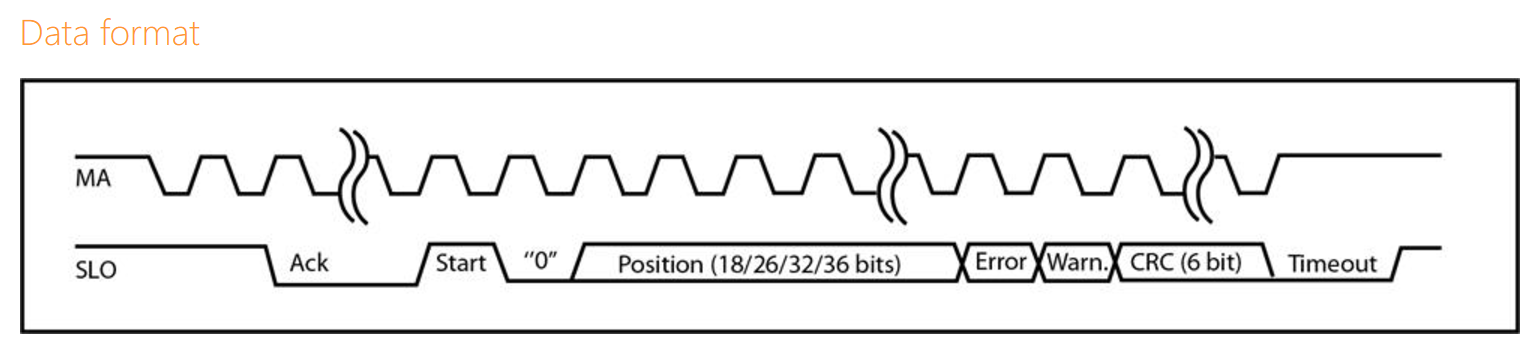
\includegraphics{pictures/ramka)danych.png}}
    \label{fig:PPLogo}
    \caption{Ramka danych protokołu Biss-C \cite{bissC2}}
\end{figure}

\noindent Dodatkową zaletą protokołu jest jego odporność na zakłócenia elektromagnetyczne czyniąc go odpowiednim rozwiązaniem nawet w trudnych warunkach przemysłowych. Istnieją również wersje rozszerzone tego protokołu zalecane do wykorzystania ze względu na bezpieczeństwo. Takim przykład jest rodzaj BiSS Safety umożliwiający spełnienie rygorystycznych norm, w tym ISO 13849 oraz IEC 61508 \cite{normy}. 

%%%%%%%%%%%%%%%%%%%%%%%%%%%%%%%%%% TEORIA %%%%%%%%%%%%%%%%%%%%%%%%%%%%%%%%%%%%%%%

%%%%%%%%%%%%%%%%%%%%%%%%%%%%%%%%%% TEORIA2 %%%%%%%%%%%%%%%%%%%%%%%%%%%%%%%%%%%%%%

%%%%%%%%%%%%%%%%%%%%%%%%%%%%%%%%%% TEORIA2 %%%%%%%%%%%%%%%%%%%%%%%%%%%%%%%%%%%%%%

%%%%%%%%%%%%%%%%%%%%%%%%%%%%%%%%%% KOD %%%%%%%%%%%%%%%%%%%%%%%%%%%%%%%%%%%%%%%
\section{Implementacja w programie}

\indent Z uwagi na budowę ramki do odczytu danych z enkodera zaimplementowano kod oddzielający kolejne sekcje krok po kroku. Poszczególne zbiory bitów zapisywanie w zależności od taktowania sygnału zegarowego są wyłapywane przez funkcje utworzone w programie powstałego na podstawie algorytmu odbierania danych z rys. \ref{fig:Blank board (1)}:

\begin{figure}[!htb]
    \centering
    \resizebox{14cm}{!}{
    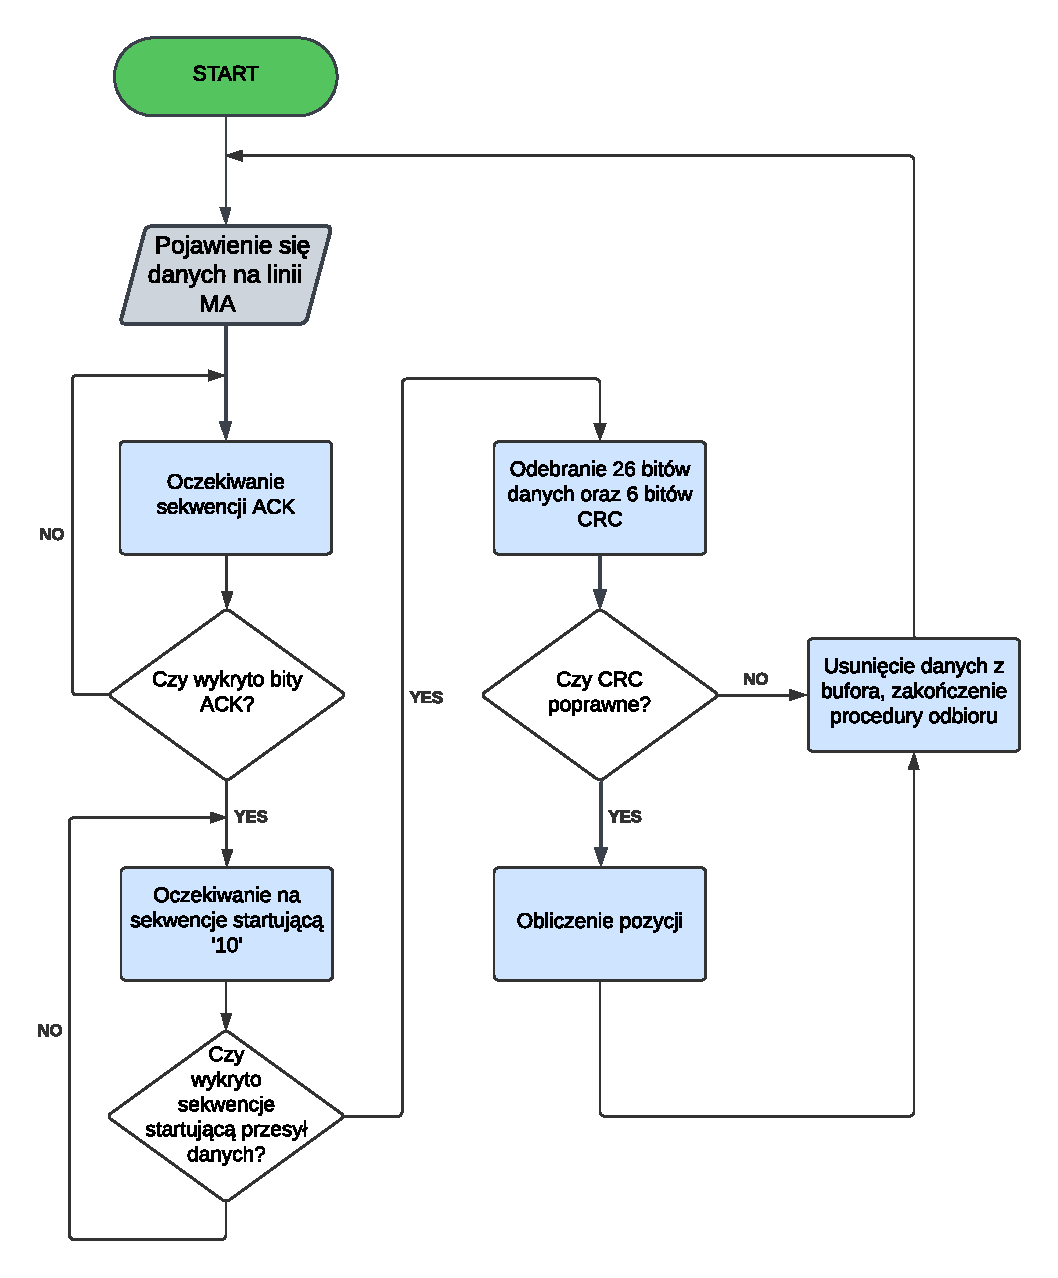
\includegraphics{pictures/Blank board (2).pdf}}
    \caption{Algorytm odbioru danych z enkodera}
    \label{fig:Blank board (1)}
\end{figure}

\vspace{0.5cm}

\newpage 

\begin{center}
    \textbf{Opis algorytmu}
\end{center}

\vspace{0.5cm}

\begin{enumerate}
    \item Oczekiwanie sekwencji ACK \newline
    Program nasłuchuje linię danych i czeka na pierwszą część ramki, czyli kod ACK. W naszym przypadku funkcja za to odpowiedzialna iteruje 8 możliwych przesunięć bitowych pierwszego bajtu bufora danych szukając miejsca, w którym sygnał wysoki z linii zmieni się na niski. Dokładniej, wynik przesunięcia jest sprawdzany z maską 0x80 w ramach operacji logicznej XOR oczkując rezultatu 0x00. Następnie ustawia zmienną programową o nazwie \textit{isAckDetected} na 1, co pozwala przejść dalej w działaniu programu

\vspace{0.5cm}

    \item Wyznaczanie bitu startu \newline
    W tym przypadku przechodzimy do znalezienia indeksu bajtu, od którego zaczyna się właściwa ramka danych poszukując początkowego wzorca bitowego $10$. Iterując cały bufor danych od momentu wykrycia ACK funkcja szuka pierwszego bajtu, który jest różny niż 0x00 stanowiąc prawdopodobnie początek głównych danych potrzebnych do odczytania położenia.

\vspace{0.5cm}
    
    \item Przesunięcie ramki bitów \newline
    Obliczane jest przesunięcie bitowe potrzebne do prawidłowego odczytu danych oraz weryfikuje początek ramki. Początkowo funkcja zaczyna sprawdzać czy poprawnie wykryto bit startu po przesunięciu ramki do indeksu z poprzedniego kroku. Sprawdza następne dwa bity $10$ za pomocą maski 0xC0, aby upewnić się, czy początek ramki jest poprawny. Jeśli początek został wykryty, flaga programowa \textit{isStartDetected} ustawia się na 1 i obliczane jest dokładne przesunięcie. Do indeksu danych dodaje się wartość 2 w celu odczytania bitów danych.

\vspace{0.5cm}
    \item Przypisanie bitów do bufora \newline 
    Przypisuje dane do struktury reprezentującej ramkę danych. Iteruje przez długość bufora ramki z enkodera przesuwając odpowiednie fragmenty danych oraz przypisując bity do docelowej struktury danych gotowej do przeliczania aktualnego położenia. Każdy element bufora ramki jest składany z dwóch sąsiednich bajtów enkodera, uwzględniając przesunięcie bitowe. Następnie cała ramka danych jest kopiowana do struktury za pomocą rzutowania.

\vspace{0.5cm}
    \newpage
    \item Obliczanie pozycji \newline
     Funkcja oblicza rzeczywistą pozycję enkodera, uwzględniając kalibrację mechaniczną i parametry enkodera. Spośród pozyskanej ramki danych wartość surowa wartości położenia zostaje zdekodowana oraz przemnożona przez współczynnik konwersji impulsów odczytanego z dokumentacji technicznej urządzenia. Końcowa wartość pozycji zostaje skorygowana o ustawiony wcześniej offset oraz przypisana do zmiennej wspomagającej sterowanie.

\vspace{0.5cm}

    \item Obliczanie sumy CRC \newline
    W celu kontroli poprawności ramki danych obliczona zostaje suma CRC, której wartość decyduje o odrzuceniu otrzymanego wyniku w zależności od ustawionej kombinacji.    
\end{enumerate}

\newpage

%%%%%%%%%%%%%%%%%%%%%%%%%%%%%%%%%% KOD %%%%%%%%%%%%%%%%%%%%%%%%%%%%%%%%%%%%%%%